   
\documentclass[11pt]{article}
\usepackage{fancyhdr}
\usepackage{extramarks}
\usepackage{amsmath}
\usepackage{amsthm}
\usepackage{thmtools}
\usepackage{amsfonts}
\usepackage{tikz}
\usepackage{algpseudocode}
\usepackage{listings}
\usepackage{enumitem}
\usepackage{float}
\usepackage[linesnumbered,ruled]{algorithm2e}

\usetikzlibrary{automata,positioning}
\renewcommand{\arraystretch}{1.25}
%
% Basic Document Settings
%

\topmargin=-0.45in
\evensidemargin=0in
\oddsidemargin=0in
\textwidth=6.5in
\textheight=9.0in
\headsep=0.25in

\linespread{1.1}

\pagestyle{fancy}
\fancyhf{}
\lhead{\hmwkAuthorName}
\chead{\hmwkClass\ : \hmwkTitle}
\rhead{\thepage}
\cfoot{\thepage}

\renewcommand\headrulewidth{0.4pt}
\renewcommand\footrulewidth{0.4pt}

\setlength\parindent{0pt}

\newcommand{\hmwkTitle}{Study Guide}
\newcommand{\hmwkClass}{CS235: Languages and Automata}
\newcommand{\hmwkAuthorName}{\textbf{Sophiya Chiang}}

\theoremstyle{definition}
\newtheorem{defn}{Definition}[section]
\newtheorem{thm}{Theorem}[section]
\newtheorem{cor}{Corollary}[thm]
\newtheorem{lemma}[thm]{Lemma}

%todo command
\newcommand{\todo}{\textcolor{red}}


% Document begins here %
\begin{document}
 

\title{
    \vspace{2in}
    \textmd{\textbf{\hmwkClass:\ \hmwkTitle}}\\
    \normalsize\vspace{0.1in}\small{Last updated: \today}\\
    \vspace{3in}
}

\author{\hmwkAuthorName}
\date{}

\maketitle

\pagebreak

\tableofcontents

\pagebreak

\section{Automata Theory}
\subsection{Regular languages}
\subsubsection{Finite automata}
\begin{itemize}[leftmargin=*]
    \item A language is called a \textbf{\textit{regular language}} if some finite automaton recognizes it
    \item If $A$ is the set of all strings that machine $M$ accepts, we say that $A$ is the \textbf{\textit{language of machine $M$}}, such that $L(M)=A$. $M$ recognizes $A$ or $M$ accepts $A$.
    \item Deterministic computation: when the machine is in a given state and reads the next input symbol, we know what the next state will be.
\end{itemize}
\begin{defn}
A \textbf{\textit{finite automaton}} is a 5-tuple $(Q,\Sigma, \delta, q_0, F)$, where
\begin{enumerate}
    \item $Q$ is a finite set called the states 
    \item $\Sigma$ is a finite set called the alphabet
    \item $\delta: Q\times\Sigma \longrightarrow Q$ is the transition function. Takes a state and an input symbol and produces the next state.
    \item $q_0 \in Q$ is the start state
    \item $F\subseteq Q$ is the set of accept states/finite states
\end{enumerate}
\end{defn}
\begin{defn}
$M$ \textbf{\textit{recognizes language}} $A$ if $A=\{w |\ M$ accepts $w\}$, where computation is defined as follows. Let $M = (Q,\Sigma, \delta, q_0,F)$ be a finite automaton and let $w=w_1w_2\ldots w_n$ be a string where each $w_i$ is a member of the alphabet $\Sigma$. Then $M$ accepts $w$ if a sequence of states $r_0,r_1,\ldots r_n \in Q$ exists with the three conditions:
\begin{enumerate}
    \item $r_0 = q_0$. (Machine starts in the start state) 
    \item $\delta(r_i, w_{i+1} = r_{i+1}$ for $i = 0, \ldots, n-1$ (Machine goes from state to state according to the transition function.
    \item $r_n \in F$. The machine accepts if its input if it ends up in an accept state.
\end{enumerate}
\end{defn}
\textbf{\underline{The regular operations}}
\begin{itemize}[leftmargin=*]
    \item Regular operations include union, concatenation and star.
    \item Unary operations apply to a single language, binary operations apply to two different languages
\end{itemize}
\begin{defn}
\textbf{Union operation:} $A\cup B = \{x\ |\ x\in A \lor x\in B\}$
\end{defn}
\begin{defn}
\textbf{Concatenation operation:} $A\circ B = \{xy\ |\ x\in A \land y\in B\}$. Attaching a string from $A$ in front of a string from $B$ in all possile ways to get the strings in the new language.
\end{defn}
\begin{defn}
\textbf{Star operation:} $A^{*} = \{x_1x_2\ldots x_k\ |\ k\geq 0 \land \forall x_i \in A\}$. Attach any number of strings in $A$ together to get a string in the new language. Empty string $\epsilon$ is a member of $A$, regardless of $A$.
\end{defn}

\begin{thm}
The class of regular languages is closed under the union operation.
\end{thm}
\begin{proof}
    Let $M_1$ recognize $A_1$, where $M_1 = (Q_1, \Sigma, \delta_1, q_1, F_1)$, and $M_2$ recognize $A_2$, where $M_2 = (Q_2, \Sigma, \delta_2, q_2, F_2)$.\\\\
    Construct $M$ to recognize $A_1 \cup A_2$, where $M = (Q, \Sigma, \delta, q_0, F)$.
    \begin{enumerate}
        \item $Q=\{(r_1,r_2)\ |\ r_1\in Q_1, r_2\in Q_2$.\\
        This set is the Cartesian product of sets $Q_$1 and $Q_2$ and is written $Q_1 \times Q_2$. It is the set of all pairs of states, the first from $Q_1$ and the second from $Q_2$.
        \item $\Sigma = \Sigma_1 \ cup \Sigma_2$, which in this case is just $\Sigma$.
        \item $\delta$, the transition function, is defined as follows. For each $(r_1,r_2)\in Q$ and each $a\in \Sigma$, let
        \begin{center}
            $\delta((r_1,r_2),a) = (\delta_1(r_1,a),\delta_2(r_2,a))$.
        \end{center}
        \item $q_0 = (q_1,q_2)$.
        \item $F$ is the set of pairs in which either member is an accept state of $M_1$ or $M_2$. We can write it as
        \begin{center}
            $F =\{(r_1,r_2)\ |\ r_1 \in F_1$ or $r_2 \in F_2\}$ or\\
            $F = (F_1 \times Q_2) \cup (Q_1 \times F_2)$.
        \end{center}
    \end{enumerate}
\end{proof}

\begin{thm}
The class of regular languages is closed under the concatenation operation.\\
(Proved in nondeterminism)
\end{thm}

\subsubsection{Nondeterminism}
\textbf{\underline{Differences between DFA and NFA}}
    \begin{enumerate}
        \item Every state of DFA always has exactly one exiting transition arrow for each symbol of the alphabet. In NFA, a state may have zero, one, or more exiting arrows for each alphabet symbol.
        \item In DFA, labels on the transition arrows are symbols from the alphabet. An NFA may have arrows labeled with more than or equal to one member of the alphabet, or the empty string $\epsilon$.
    \end{enumerate}
\begin{itemize}[leftmargin=*]
    \item A generalization of determinism, so every deterministic finite automaton (DFA) is a non-deterministic finite automaton (NFA).
    \item Nondeterminism is akin to a kind of "parallel computation" wherein multiple independent processes or threads can be running concurrently. 
    \item When the NFA splits to follow several choices, it corresponds to a process forking into several children each proceeding separately.
    \begin{figure}[h]
    	\centering
    	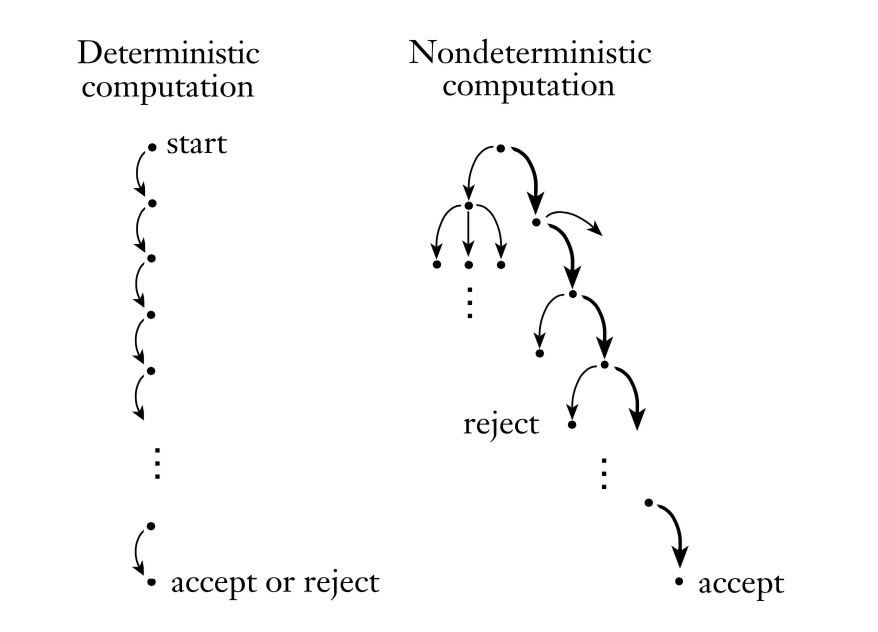
\includegraphics[width=0.5\linewidth]{nfa.png}
    	\caption{Deterministic and nondeterministic computations with an accepting branch}
    	\label{fig}
    \end{figure}
    \item Formal definition of NFA differs from DFA in the type of transition function. In NFA, the transition function takes a state and an input symbol (or empty string), and produces the \textit{set of possible states.}
\end{itemize}
\begin{defn}
A \textbf{\textit{nondeterministic finite automaton}} is a 5-tuple $(Q,\Sigma, \delta, q_0, F)$, where
\begin{enumerate}
    \item $Q$ is a finite set called the states 
    \item $\Sigma$ is a finite alphabet
    \item $\delta: Q\times\Sigma_\epsilon \longrightarrow \wp(Q)$ is the transition function. Takes a state and an input symbol and produces the set of possible states (The power set). And $\Sigma_\epsilon = \Sigma\cup\{\epsilon\}$.
    \item $q_0 \in Q$ is the start state
    \item $F\subseteq Q$ is the set of accept states
\end{enumerate}
\end{defn}

\textbf{\underline{Equivalence of NFAs and DFAs}}
\begin{thm}
Every nondeterministic finite automaton has an equivalent deterministic finite automaton.
\end{thm}
\begin{proof}
    Let $N = (Q, \Sigma, \delta, q_0 , F)$ be the NFA recognizing some language $A$. We construct a DFA $M =(Q',\Sigma,\delta',q_0',F')$ recognizing $A$.Before doing the full construction, let's first consider the easier case wherein $N$ has no $\epsilon$ arrows. Later we take the $\epsilon$ arrows into account.
    \begin{enumerate}
        \item $Q' = P(Q)$\\
        Every state of $M$ is a set of states of $N$.
        \item For $R \in Q'$ and $a \in \Sigma$, let $\delta'(R, a) = \{q \in Q\ |\ q \in \delta(r, a)$ for some $r \in R\}$. If $R$ is a state of $M$, it is also a set of states of $N$. When $M$ reads a symbol $a$ in state $R$, it shows where $a$ takes each state in $R$. Because each state may go to a set of states, we take the union of all these sets. Another way to write this expression is
        \begin{center}
            $\delta'(R,a) = \bigcup_{r\in R} \delta(r,a)$
        \end{center}
        \item $q_0'=\{q_0\}$. $M$ starts in the state corresponding to the collection containing just the start state of $N$.
        \item $F' = \{R\in Q'\ |\ R$ contains an accept state of $N\}$.\\
        The machine M accepts if one of the possible states that N could be in at this point is an accept state.
    \end{enumerate}
    Now we need to consider the $\epsilon$ arrows. To do so, we set up an extra bit of notation.For any state $R$ of $M$, we define $E(R)$ to be the collection of states that can be reached from members of $R$ by going only along $\epsilon$ arrows, including the members of $R$ themselves. Formally, for $R \subseteq Q$ let 
    \begin{center}
        $E(R) = \{q\ |\ q$ can be reached from $R$ by traveling along 0 or more $\epsilon$ arrows$\}$.
    \end{center}
    Then we modify the transition function of $M$ to account for all states that can be reached by going along $\epsilon$ arrows after every step. Replacing $\delta'(r,a)$ by $E(\delta(r, a))$ achieves this effect. Thus
    \begin{center}
        $\delta'(R,a) = \{q\in Q\ |\ q\in E(\delta(r,a))$ for some $r\in R\}$.
    \end{center}
    Additionally, we need to modify the start state of $M$ to account for all possible states that can be reached from the start state of $N$ along the $\epsilon$ arrows. Changing $q_0'$ to be $E(\{q_0\})$ achieves this effect. We have now completed the construction of the DFA $M$ that simulates the NFA $N$.
    The construction of $M$ works correctly. At every step in the computation of $M$ on an input, it clearly enters a state that corresponds to the subset of states that $N$ could be in at that point. Thus our proof is complete.
\end{proof}
\begin{cor}
    A language is regular $\iff$ some nondeterministic finite automaton recognizes it.
\end{cor}
\begin{proof}
One direction of the "if and only if" condition states that a language is regular if some NFA recognizes it. By the previous theorem, we know that any NFA can be converted into an equivalent DFA. Consequently, if an NFA recognizes some language, so does some DFA, and hence the language is regular. The other direction of the "if and only if" condition states that a language is regular only if some NFA recognizes it. That is, if a language is regular, some NFA must be recognizing it. Obviously, this condition is true because a regular language has a DFA recognizing it and any DFA is also an NFA.
\end{proof}

\textbf{\underline{Closure under the regular operations}}\\
Using nondeterminism, we can prove that the class of regular languages are closed under the regular operations such as union, concatenation, and star.
\begin{thm}
The class of regular languages is closed under the union operation.
\end{thm}
\begin{proof}
    Let $N_1 = (Q_1, \Sigma, \delta_1, q_1, F_1)$ recognize $A_1$, and $N_2= (Q_2, \Sigma, \delta_2, q_2, F_2)$ recognize $A_2$.\\\\
    Construct $N = (Q, \Sigma, \delta, q_0, F)$ to recognize $A_1\cup A_2$.
    \begin{enumerate}
        \item $Q = \{q_0\} \cup Q_1 \cup Q_2$. The states of $N$ are all the states of $N_1$ and $N_2$, with the addition of a new start state $q_0$.
        \item The state $q_0$ is the start state of $N$.
        \item The set of accept states $F=F_1\cup F_2$. The accept states of $N$ are all the accept states of $N_1$ and $N_2$. That way, $N$ accepts if either $N_1$ accepts or $N_2$ accepts.
        \item Define $\delta$ so that for any $q\in Q$ and $a\in \Sigma_\epsilon$:
        \begin{equation*}
            \delta(q,a) = \begin{cases}
               \delta_1(q,a)               & q\in Q_1\\
               \delta_2(q,a)               & q\in Q_2\\
               \{q_1,q_2\}               & q = q_0 \text{ and } a=\epsilon\\
               \emptyset               & q = q_0 \text{ and } a\neq\epsilon.
           \end{cases}
\end{equation*}
    \end{enumerate}
\end{proof}
\begin{figure}[h]
	\centering
	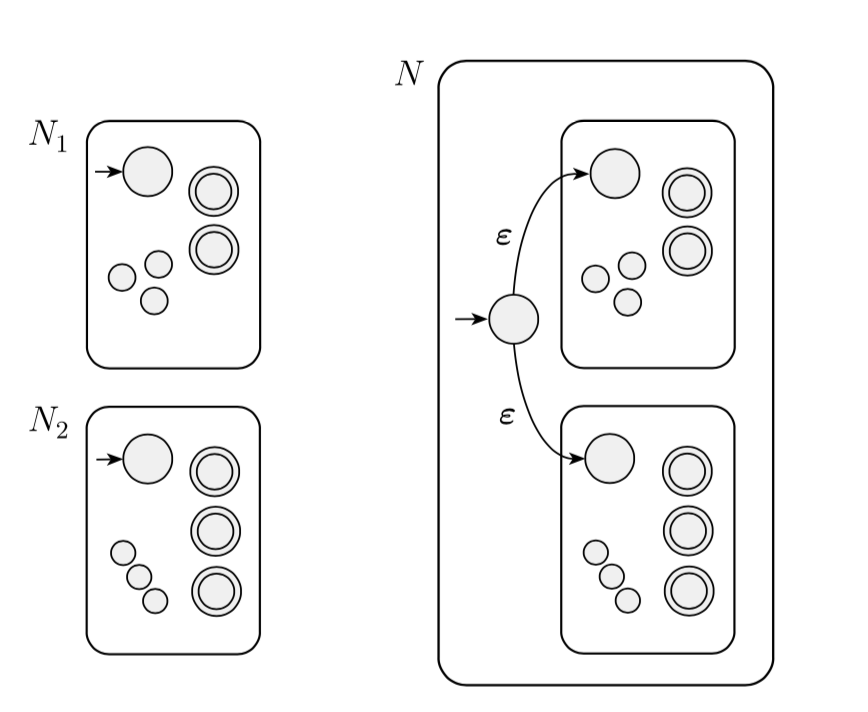
\includegraphics[width=0.5\linewidth]{nfa_union.png}
	\caption{Construction of NFA $N$ to recognize $A_1\cup A_2$}
	\label{fig}
\end{figure}

\begin{thm}
The class of regular languages is closed under the concatenation operation.
\end{thm}
\begin{proof}
Let $N_1 = (Q_1, \Sigma, \delta_1, q_1, F_1)$ recognize $A_1$, and $N_2= (Q_2, \Sigma, \delta_2, q_2, F_2)$ recognize $A_2$.\\\\
Construct $N = (Q, \Sigma, \delta, q_0, F)$ to recognize $A_1\circ A_2$.
\begin{enumerate}
    \item $Q = Q_1 \cup Q_2$.\\
    The states of $N$ are all the states of $N_1$ and $N_2$.
    \item The state $q_1$ is the same as the start state of $N_1$.
    \item The set of accept states $F_2$ are the same as the accept states of $N_2$.
    \item Define $\delta$ so that for any $q\in Q$ and $a\in \Sigma_\epsilon$:
    \begin{equation*}
        \delta(q,a) = \begin{cases}
           \delta_1(q,a)               & q\in Q_1 \text{ and } q\notin F_1\\
           \delta_1(q,a)               & q\in F_1 \text{ and } a\neq\epsilon\\
           \delta_1(q,a)\cup\{q_2\}    & q\in F_1 \text{ and } a=\epsilon\\
           \delta_2(q,a)               & q\in Q_2.
       \end{cases}
    \end{equation*}
    \end{enumerate}   
\end{proof}
\begin{figure}[h]
	\centering
	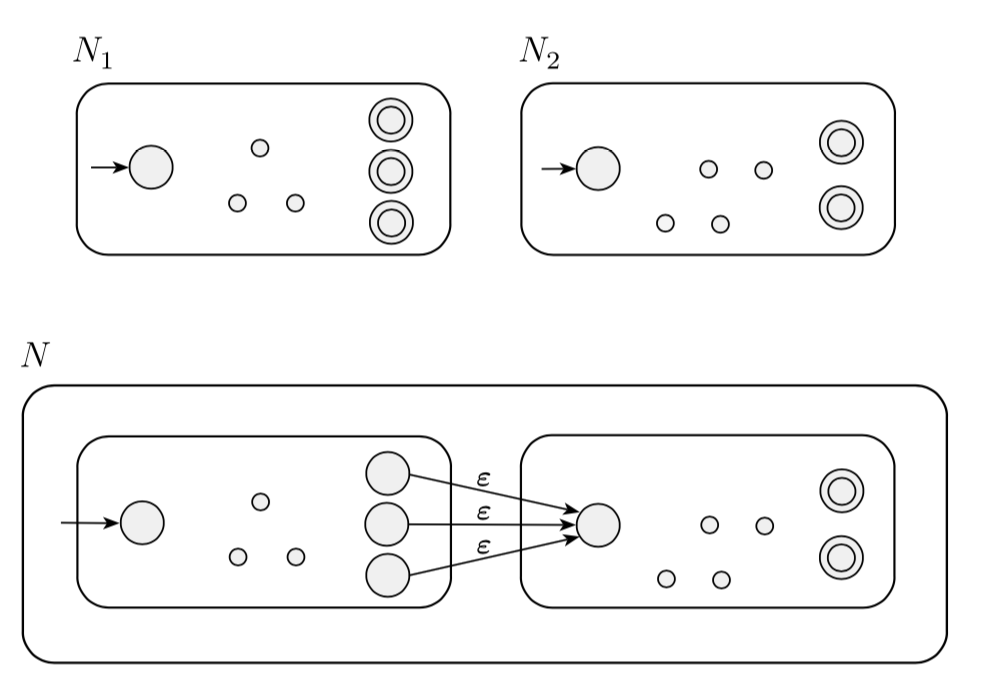
\includegraphics[width=0.5\linewidth]{nfa_concat.png}
	\caption{Construction of NFA $N$ to recognize $A_1\circ A_2$}
	\label{fig}
\end{figure}

\begin{thm}
The class of regular languages is closed under the star operation.
\end{thm}
\begin{proof}
    Let $N_1 = (Q_1, \Sigma, \delta_1, q_1, F_1)$ recognize $A_1$.\\\\
    Construct $N = (Q, \Sigma, \delta, q_0, F)$ to recognize $A_1^*$.
    \begin{enumerate}
        \item $Q = \{q_0\}\cup Q_1$.\\
        The states of $N$ are the states of $N_1$ and new start state $q_0$.
        \item The state $q_0$ is the start state of $N$.
        \item $F = \{q_0\}\cup F_1$.\\
        The set of accept states are the old accept states plus the new start state.
        \item Define $\delta$ so that for any $q\in Q$ and $a\in \Sigma_\epsilon$:
        \begin{equation*}
            \delta(q,a) = \begin{cases}
               \delta_1(q,a)               & q\in Q_1 \text{ and } q\notin F_1\\
               \delta_1(q,a)               & q\in F_1 \text{ and } a\neq\epsilon\\
               \delta_1(q,a)\cup\{q_1\}    & q\in F_1 \text{ and } a=\epsilon\\
                \{q_1\}               & q = q_0 \text{ and } a=\epsilon\\
               \emptyset               & q = q_0 \text{ and } a\neq\epsilon.
           \end{cases}
        \end{equation*}
    \end{enumerate}   
\end{proof}
\begin{figure}[h]
	\centering
	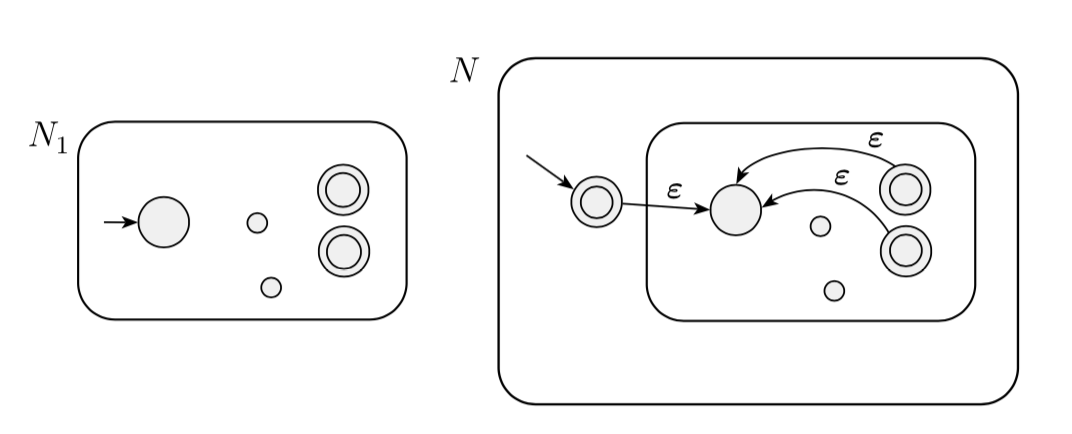
\includegraphics[width=0.5\linewidth]{nfa_star.png}
	\caption{Construction of NFA $N$ to recognize $A^*$}
	\label{fig}
\end{figure}
\subsubsection{Regular expressions}
\begin{defn}
Say that $R$ is a \textbf{\textit{regular expression}} if $R$ is
\begin{enumerate}
    \item $a$ for some $a\in \Sigma$ 
    \item $\epsilon$ 
    \item $\emptyset$
    \item $(R_1\cup R_2)$ where $R_1, R_2$ are regular expressions
    \item $(R_1\circ R_2)$ where $R_1, R_2$ are regular expressions, or
    \item $(R_1^{*})$ where $R_1$ is a regular expression.
\end{enumerate}
In items 1 and 2, the regular expressions $a$ and $\epsilon$ represent the languages $\{a\}$ and $\{\epsilon\}$, respectively. In item 3, the regular expression $\emptyset$ represents the empty language. In items 4, 5, and 6, the expressions represent the languages obtained by taking the union or concatenation of the languages $R_1$ and $R_2$, or the star of the language $R_1$, respectively.
\end{defn}
\textbf{\underline{Equivalence with finite automata}}
\begin{thm}
A language is regular $\iff$ some regular expression describes it.
\end{thm}
\begin{lemma}
    If a language is described by a regular expression, then it is regular.
\end{lemma}
\begin{proof}
\textit{This is the procedure to convert a regular expression to a corresponding $NFA$.}\\
Let's convert $R$ into an NFA $N$. We consider the six cases in the formal definition of regular expressions.
\begin{enumerate}
    \item $R = a$ for some $a \in\Sigma$. Then $L(R) = \{a\}$, and the following NFA recognizes $L(R)$.
    \begin{figure}[h]
	\centering
	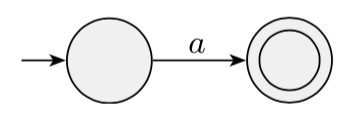
\includegraphics[width=0.3\linewidth]{proc1.png}
	\label{fig}
\end{figure}

    \item $R=\epsilon$. Then $L(R)=\epsilon$, and the following NFA recognizes $L(R)$.
        \begin{figure}[H]
	\centering
	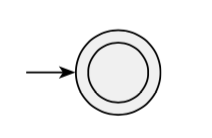
\includegraphics[width=0.2\linewidth]{proc2.png}
	\label{fig}
\end{figure}

    \item $R=\emptyset$. Then $L(R)=\emptyset$, and the following NFA recognizes $L(R)$.
    \begin{figure}[H]
	\centering
	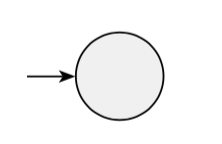
\includegraphics[width=0.2\linewidth]{proc3.png}
	\label{fig}
    \end{figure}

    \item $R = R_1\cup R_2$.
    \item $R = R_1\circ R_2$.
    \item $R = R_1^*$.
\end{enumerate}
\end{proof}

\begin{defn}
A \textbf{\textit{generalized nondeterministic finite automaton}} (GNFA) is a 5-tuple $(Q,\Sigma, \delta, q_{start}, q_{accept})$, where
\begin{enumerate}
    \item $Q$ is a finite set called the states 
    \item $\Sigma$ is the input alphabet
    \item $\delta: (Q-\{q_{accept}\})\times(Q-\{q_{start}\}) \longrightarrow R$ is the transition function, where $R$ is the collection of all regular expressions over the alphabet $\Sigma$
    \item $q_{start}$ is the start state
    \item $q_{accept}$ is the accept state
\end{enumerate}

General GNFA rules:
\begin{itemize}
    \item The start state has transition arrows going to every other state but no arrows coming in from any other state.
    \item There is only a single accept state, and it has arrows coming in from every other state but no arrows going to any other state. Furthermore, the accept state is not the same as the start state.
    \item Except for the start and accept states, one arrow goes from every state to every other state and also from each state to itself.
\end{itemize}
\end{defn}

\begin{lemma}
If a language is regular, then it is described by a regular expression.
\end{lemma}
\begin{proof}
    \textit{This is the procedure to convert a DFA into equivalent regular expression.}\\
    \begin{figure}[H]
	\centering
	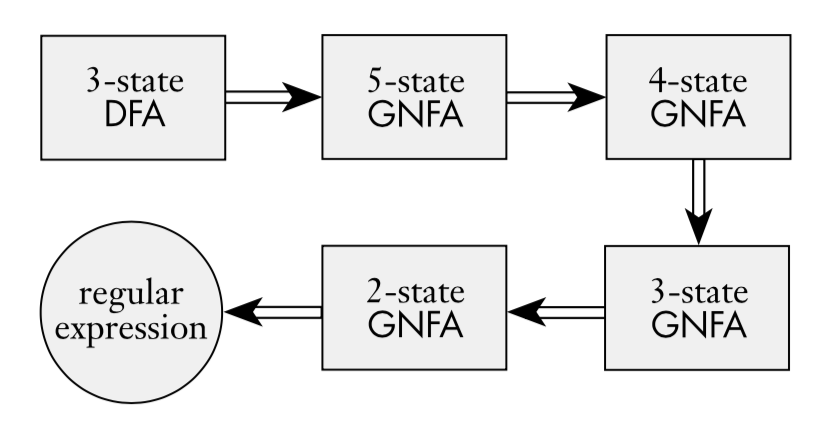
\includegraphics[width=0.4\linewidth]{GNFA.png}
	\caption{Example stages in converting a DFA to a regular expression}
	\label{fig}
    \end{figure}
    To convert a DFA to a GNFA:
    \begin{enumerate}
        \item Add new start state with $\epsilon$ arrow to old start state.
        \item Add new accept state with $\epsilon$ arrows from old accept states.
        \item Remove old accept states.
        \item Multiple labels on arrow are replaced by union of labels.
    \end{enumerate}
    From GNFA to regular expression, we simply go state by state and rip it out from the machine, as long as the state is not the start or accept state.
\end{proof}

\subsubsection{Nonregular languages}
\textbf{\underline{The pumping lemma for regular languages}}
\begin{thm}
    If $A$ is a regular language, then there is a number $p$ (the pumping length) where if $s$ is any string in $A$ of length at least $p$, then $s$ may be divided into three pieces, $s = xyz$, satisfying the following conditions:
    \begin{enumerate}
        \item for each $i\geq 0, xy^iz\in A$,
        \item $|y|>0$, and
        \item $|xy| \leq p$.
    \end{enumerate}
When $s$ is divided into $xyz$, either $x$ or $z$ may be $\epsilon$, but condition 2 says that $y \neq \epsilon$. $x$ and $y$ together have length at most $p$.
\end{thm}

\subsection{Context-free languages}
\subsubsection{Context-free grammars}
\begin{itemize}[leftmargin=*]
    \item A grammar consists of a collection of \textbf{substitution rules}, aka \textbf{productions}.
    \item A \textbf{derivation} is the sequence of substitutions to obtain a string. The same information can be represented as a \textbf{parse tree}.
    \item Yields: $uAv \Rightarrow uwv$
    \item $u$ derives $v$: ($u\overset{*}{\Rightarrow}v$), if $u=v$ or if a sequence of $u_1,u_2,\ldots,u_k$ exists for some $k\leq0$ and $u\Rightarrow u_1\Rightarrow u_2\Rightarrow\ldots\Rightarrow u_k\Rightarrow v$.
    \item The language of the grammar is $\{w \in \Sigma^{^{*}}\ |\ S \Rightarrow^{^{*}} w\}$.
    \item If a language can only be generated by ambiguous grammars, then the language is \textbf{inherently ambiguous}.
\end{itemize}
\begin{defn}
A \textbf{\textit{context-free grammar}} is a 4-tuple $(V,\Sigma,R,S)$, where
\begin{enumerate}
    \item $V$ is a finite set called the variables,
    \item $\Sigma$ is a finite set, disjoint from $V$, called the terminals,
    \item $R$ is a finite set of rules, with each rule being a variable and a string of variables and terminals, and
    \item $S\in V$ is the start variable
\end{enumerate}
\end{defn}

\begin{defn}
A string $w$ is derived ambiguously in context-free grammar $G$ if it has two or more different leftmost derivations. Grammar $G$ is ambiguous if it generates some string ambiguously.
\end{defn}
\textbf{\underline{Chomsky Normal Form}}
\begin{defn}
A context-free grammar is in \textbf{Chomsky normal form} if every rule is
of the form
    \begin{center}
        $A \to BC$\\
        $A \to a$
    \end{center}
where $a$ is any terminal and $A, B,$ and $C$ are any variables, except that $B$ and $C$ may not be the start variable. In addition, we permit the rule $S\to \epsilon$, where $S$ is the start variable.
\end{defn}
\begin{itemize}[leftmargin=*]
    \item For any string $w\in L(G)$ of length $n\geq 1$, exactly $2n-1$ steps are required for the derivation of $w$, if $G$ is in Chomsky Normal Form (CNF)
\end{itemize}
\begin{thm}
    Any context-free language is generated by a context-free grammar in Chomsky
normal form.
\end{thm}
\begin{proof}
We can convert any grammar $G$ into CNF:
\begin{enumerate}
    \item Add a new start variable $S_0\to S$
    \item Eliminate all $\epsilon$-rules: remove an $\epsilon$-rule $A\to \epsilon$
    \item Eliminate all unit-rules. We remove a unit rule $A \to B$. Then, whenever a rule $B \to u$ appears, we add the rule $A \to u$ unless this was a unit rule previously removed. As before, $u$ is a string of variables and terminals. We repeat these steps until we eliminate all unit rules.
    \item Convert all remaining rules into proper form.
\end{enumerate}
\end{proof}

\subsubsection{Pushdown automata}
\begin{itemize}[leftmargin=*]
    \item Pushdown automata are equivalent in power to context-free grammars.
    \item A schematic representation of a pushdown automaton. The control represents the states and transition function, the tape contains the input string, and the arrow represents the input head, pointing at the next input symbol to be read. The pushdown automaton has a \textbf{stack} component, which provides additional memory beyond the finite amount available in the control.
    \begin{figure}[H]
    	\centering
    	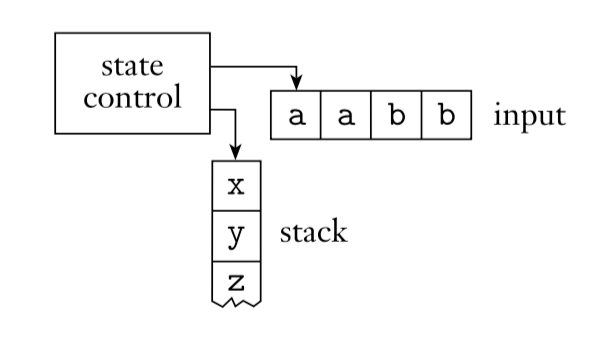
\includegraphics[width=0.5\linewidth]{pda.png}
    	\caption{Schematic of a pushdown automaton}
    	\label{fig}
    \end{figure}
    \item Pushing a symbol: Writing a symbol on the stack tape.
    \item Popping a symbol: Removing a symbol from the stack tape.
    \item A stack is a last-in-first-out storage device.
\end{itemize}
\begin{defn}
A \textbf{\textit{pushdown automaton}} is a 6-tuple $(Q,\Sigma, \Gamma, \delta, q_0, F)$, where $Q,\Sigma, \Gamma,  F$ are all finite sets, and
\begin{enumerate}
    \item $Q$ is the set of states
    \item $\Sigma$ is the input alphabet
    \item $\Gamma$ is the stack alphabet
    \item $\delta:Q\times\Sigma_\epsilon\times \Gamma_\epsilon\to \wp(Q\times\Gamma_\epsilon$ is the transition function
    \item $q_0\in Q$ is the start state, and 
    \item $F\subseteq Q$ is the set of accept states.
\end{enumerate}
A pushdown automaton $M = (Q,\Sigma, \Gamma, \delta, q_0, F)$ computes as follows: It accepts input $w$ if $w$ can be written as $w=w_1w_2\ldots w_m$, where each $w_i\in \Sigma_\epsilon$ and sequences of states $r_0,r_1,\ldots, r_m\in Q$ and strings $s_0,s_1,\ldots,s_m\in \Gamma^*$ exist that satisfy the following conditions. The strings $s_i$ represent the sequence of stack contents that $M$ has on the accepting branch of the computation.
\begin{enumerate}
    \item $r_0 = q_0$ and $s_0 = \epsilon$. $M$ starts out properly, in the start state and with an empty stack.
    \item For $i=0,\ldots, m-1$, we have $(r_{i+1}, b)\in \delta(r_i, w_{i+1}, a)$, where $s_i = at$ and $s_{i+1} = bt$ for some $a,b\in \Gamma_\epsilon$ and $t\in\Gamma^*$. $M$ moves properly according to the state, stack, and next input symbol.
    \item $r_m\in F$. An accept state occurs at the input end.
\end{enumerate}
\end{defn}
\textbf{\underline{Equivalence with context-free grammars}}
\begin{thm}
    A language is context-free $\iff$ some pushdown automaton recognizes it.
\end{thm}
\begin{lemma}
If a language is context free, then some pushdown automaton recognizes it.
\end{lemma}
\begin{proof}
    \textit{This is the procedure to convert a context-free grammar into an equivalent PDA.}
        \begin{figure}[H]
    	\centering
    	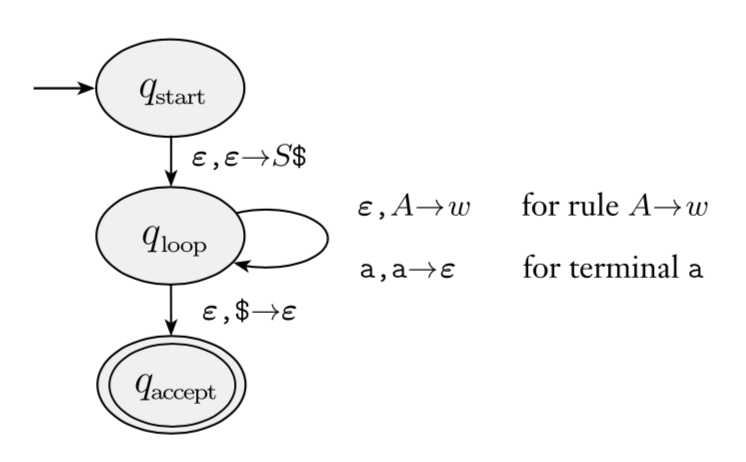
\includegraphics[width=0.5\linewidth]{CFGPDA.png}
    	\caption{State diagram of CFG to PDA conversion}
    	\label{fig}
    \end{figure}
    \begin{enumerate}
        \item Stack symbol at $q_0$: $\epsilon,\epsilon\to \$$
        \item Push starting variable to top of stack.
        \item At $q_{loop}$: push var/terminals on the RHS of all productions starting at rightmost symbol. First, replace the start symbol with rightmost symbol and keep pushing the rest of the symbols from right to left.
        \item Keep popping terminals from production.
        \item At $q_f$: Pop stack symbol $\epsilon,\$\to\epsilon$.
    \end{enumerate}
\end{proof}
\begin{lemma}
If a pushdown automaton recognizes some language, then it is context free.
\end{lemma}
\begin{proof}
    Assume without loss of generality:
    \begin{enumerate}
        \item  $P$ has a single accept state, $q_{accept}$.
        \item $P$ empties its stack before accepting.
        \item Each transition does either a push or a pop, but not both.
    \end{enumerate}
    Given the pushdown automata $P = (Q, \Sigma, \Gamma, \delta, q_0, \{q_{accept}\})$. We want to construct a context-free grammar $G$. \\
    The variables of $G$ are $V = \{A_{pq}\ |\ p, q \in Q\}$. The start variable is $S = A_{q_0 ,q_{accept}}$ . Now we describe $G$'s rules in three parts.
    \begin{enumerate}
        \item For each $p, q, r, s\in Q, u\in \Gamma$ and $a,b\in \Sigma\epsilon$, if $\delta(p,a,\epsilon)$ contains $(r,u)$ and $\delta(s,b,u)$ contains $(q,\epsilon)$, put the rule $A_{pq}\to aA_{rs}b$ in $G$.
        \item For each $p, q, r\in Q$, put the rule $A_{pq}\to A_{pr}A_{rq}$ in $G$.
        \item Finally, for each $p \in Q$, put the rule $A_{pp}\to\epsilon$ in $G$.
    \end{enumerate}
\end{proof}

\subsubsection{Non-context-free languages}
\textbf{\underline{The pumping lemma for context-free languages}}
\begin{thm}
    If $A$ is a context-free language, then there is a number $p$ (the pumping length) where if $s$ is any string in $A$ of length at least $p$, then $s$ may be divided into five pieces, $s = uvxyz$, satisfying the following conditions:
    \begin{enumerate}
        \item for each $i\geq 0, uv^ixy^iz\in A$,
        \item $|vy|>0$, and
        \item $|vxy| \leq p$.
    \end{enumerate}
When $s$ is divided into $xyz$, either $x$ or $z$ may be $\epsilon$, but condition 2 says that $y \neq \epsilon$. $x$ and $y$ together have length at most $p$.
\end{thm}
\pagebreak
\section{Computability Theory}
\subsection{Turing machines}
\begin{itemize}[leftmargin=*]
    \item Turing machines use an infinite tape as its unlimited memory.
    \item It has a tape head that can read and write symbols and move around on the tape.
    \item The schematic of a Turing Machine:
    \begin{figure}[h]
    	\centering
    	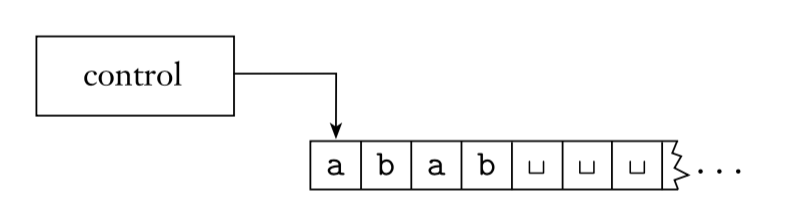
\includegraphics[width=0.5\linewidth]{tm.png}
    	\caption{Schematic of a Turing machine}
    	\label{fig}
    \end{figure}
    \item The collection of strings that a Turing machine $M$ accepts is the language or $M$, or the language recognized by $M$, denoted by $L(M)$.
\end{itemize}
\textbf{\underline{Differences between finite automata and Turing machines}}
\begin{enumerate}
    \item A Turing machine can both write on the tape and read from it.
    \item The read–write head can move both to the left and to the right.
    \item The tape is infinite.
    \item The special states for rejecting and accepting take effect immediately.
\end{enumerate}
\begin{defn}
A \textbf{\textit{Turing machine}} is a 7-tuple $(Q,\Sigma, \Gamma, \delta, q_0, q_{accept},q_{reject})$, where $Q,\Sigma, \Gamma$ are all finite sets, and
\begin{enumerate}
    \item $Q$ is the set of states
    \item $\Sigma$ is the input alphabet not containing the blank symbol $\sqcup$,
    \item $\Gamma$ is the tape alphabet, where $\sqcup\in\Gamma$ and $\Sigma\subseteq\Gamma$,
    \item $\delta:Q\times\Gamma\to Q\times\Gamma\times \{L,R\}$ is the transition function
    \item $q_0\in Q$ is the start state, 
    \item $q_{accept}\in Q$ is the accept state, and 
    \item $q_{reject}\in Q$ is the reject state.
\end{enumerate}
A Turing machine $M = (Q,\Sigma, \Gamma, \delta, q_0, q_{accept},q_{reject})$ computes as follows. Initially, $M$ receives its input $w = w_1w_2\ldots w_n \in\Sigma^*$ on the leftmost $n$ squares of the tape, and the rest of the tape is blank (i.e., filled with blank symbols). The head starts on the leftmost square of the tape. Note that $\Sigma$ does not contain the blank symbol, so the first blank appearing on the tape marks the end of the input. Once $M$ has started, the computation proceeds according to the rules described by the transition function. If $M$ ever tries to move its head to the left off the left-hand end of the tape, the head stays in the same place for that move, even though the transition function indicates L. The computation continues until it enters either the accept or reject states, at which point it halts. If neither occurs, $M$ goes on forever.\\\\
As a Turing machine computes, changes occur in the current state, the current tape contents, and the current head location. A setting of these three items is called a configuration of the Turing machine. Configurations often are represented in a special way. For a state $q$ and two strings $u$ and $v$ over the tape alphabet $\Gamma$, we write $u q v$ for the configuration where the current state is $q$, the current tape contents is $uv$, and the current head location is the first symbol of $v$. The tape contains only blanks following the last symbol of $v$. 
\end{defn}
\begin{defn}
Call a language \textbf{Turing-recognizable} if some Turing machine recognizes it.\\
Or \textbf{recursively enumerable language}.
\end{defn}
\begin{defn}
Call a language Turing-decidable or simply decidable if some Turing machine decides it.\\
Or \textbf{recursive language}.\\\\
A Turing machines that halt on all inputs, never loops. These machines are called deciders because they always make a decision to accept or reject. A decider that recognizes some language also is said to decide that language.
\end{defn}
\subsection{Variants of Turing machines}
\begin{itemize}[leftmargin=*]
    \item Variants of TMs and the original TM all have the same power because they recognize the same class of languages.
    \item Robustness: invariance to certain changes in the definition.
    \item To show two models are equivalent, we can show that one can simulate the other. If they recognize the same language then they are equivalent.
\end{itemize}
\textbf{\underline{Multitape Turing machine}}
\begin{thm}
    Every multitape Turing machine has an equivalent single-tape Turing machine.
\end{thm}
\begin{proof}
    Converting a multitape TM $M$ to an equivalent single-tape TM $S$. (Simulating $M$ with $S$)
\end{proof}
\begin{cor}
    A language is Turing-recognizable if and only if some multitape Turing machine recognizes it.
\end{cor}
\begin{proof}
    A Turing-recognizable language is recognized by an ordinary (single-tape) Turing machine, which is a special case of a multitape Turing machine. That proves one direction of this corollary.
\end{proof}
\textbf{\underline{Nondeterministic Turing machine}}
\begin{itemize}[leftmargin=*]
    \item The transition function for a nondeterministic Turing machine has the form
    \begin{center}
        $\delta:Q\times\Gamma\to\wp(Q\times\Gamma\times\{L,R\})$
    \end{center}
    \item The computation of a nondeterministic Turing machine is a tree whose branches correspond to different possibilities for the machine. 
    \item If some branch of the computation leads to the accept state, the machine accepts its input.
\end{itemize}
\begin{thm}
    Every nondeterministic Turing machine has an equivalent deterministic Turing machine.
\end{thm}
\begin{proof}
    The simulating deterministic TM $D$ has three tapes. This arrangement is equivalent to having a single tape because any multitape TM can be simulated by a single-tape TM. The machine $D$ uses its three tapes in a particular way, as illustrated in the following figure. Tape 1 always contains the input string and is never altered. Tape 2 maintains a copy of $N$'s tape on some branch of its nondeterministic computation. Tape 3 keeps track of $D$'s location in $N$'s nondeterministic computation tree.
    \begin{figure}[H]
    	\centering
    	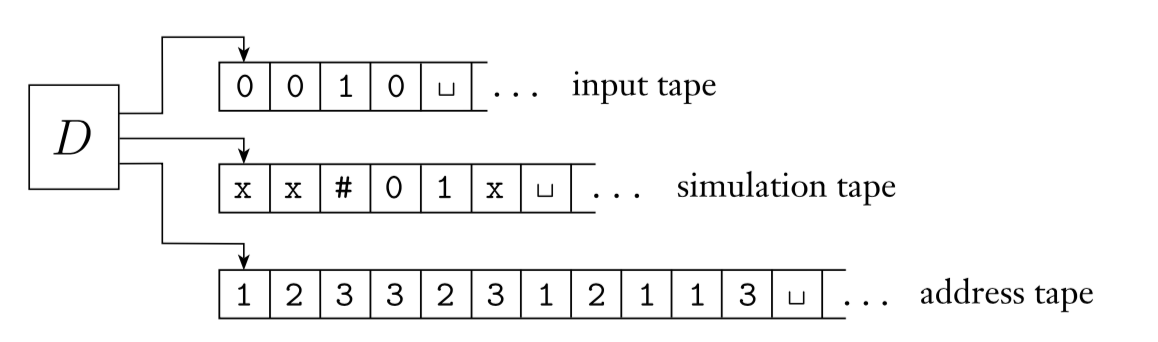
\includegraphics[width=0.5\linewidth]{ndtm.png}
    	\caption{Deterministic TM $M$ simulating nondeterministic TM $N$}
    	\label{fig}
    \end{figure}
\end{proof}
\begin{cor}
        A language is Turing-recognizable if and only if some nondeterministic Turing machine recognizes it.
\end{cor}
\begin{proof}
    Any deterministic TM is automatically a nondeterministic TM, and so one direction of this corollary follows immediately. 
\end{proof}
\begin{cor}
    A language is decidable if and only if some nondeterministic Turing machine
decides it.
\end{cor}

\textbf{\underline{Enumerators}}
\begin{itemize}[leftmargin=*]
    \item Turing-recognizable languages = recursively enumerable language
    \item An enumerator is a Turing machine with an attached printer
    \item The Turing machine can use that printer as an output device to print strings. 
    \item Every time the Turing machine wants to add a string to the list, it sends the string to the printer.
    \item An enumerator $E$ starts with a blank input on its work tape. If the enumerator doesn't halt, it may print an infinite list of strings. The language enumerated by $E$ is the collection of all the strings that it eventually prints out. 
    \item Moreover, $E$ may generate the strings of the language in any order, possibly with repetitions.
\end{itemize}
\begin{figure}[H]
	\centering
	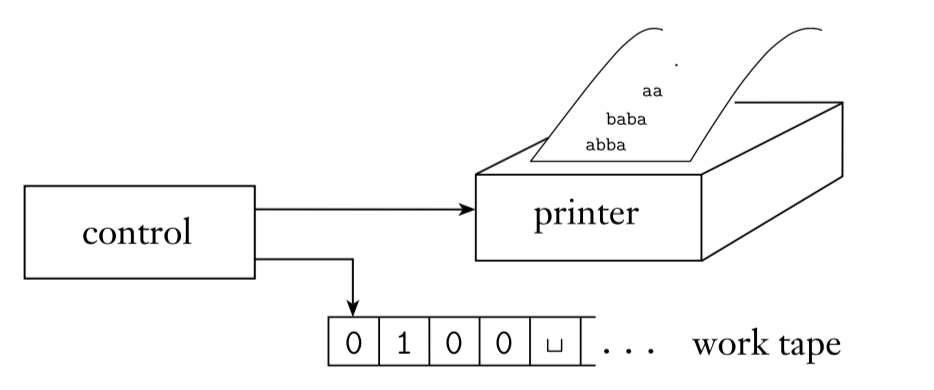
\includegraphics[width=0.5\linewidth]{enum.png}
	\caption{Schematic of a Turing machine}
	\label{fig}
\end{figure}
\begin{thm}
    A language is Turing-recognizable if and only if some enumerator enumerates it.
\end{thm}
\begin{proof}
First we show that if we have an enumerator $E$ that enumerates a language $A$, a TM $M$ recognizes $A$. The TM $M$ works in the following way.\\\\
    $M$ = "On input $w$:
    \begin{enumerate}
        \item Run $E$. Every time that $E$ outputs a string, compare it with $w$.
        \item If $w$ ever appears in the output of $E$, accept.
    \end{enumerate}
$M$ accepts those strings that appear on $E$'s list.\\
Now we do the other direction. If TM $M$ recognizes a language $A$, we can construct the following enumerator $E$ for $A$. Say that $s_1,s_2,s_3,\ldots$ is a list of all possible strings in $\Sigma^*$.\\\\
$E$ = "Ignore the input.
\begin{enumerate}
    \item Repeat the following for $i = 1, 2, 3, \ldots$
    \item Run $M$ for $i$ steps on each input $s_1,s_2,s_3,\ldots, s_i$.
    \item If any computations accept, print out the corresponding $s_j$."
\end{enumerate}
If $M$ accepts a particular string $s$, eventually it will appear on the list generated by $E$. In fact, it will appear on the list infinitely many times because $M$ runs from the beginning on each string for each repetition of step 1. This procedure gives the effect of running $M$ in parallel on all possible input strings.
\end{proof}

% \subsection{Algorithm definition}
% \begin{itemize}[leftmargin=*]
%     \item An algorithm is a collection of simple instructions for carrying out some task
% \end{itemize}

\subsection{Decidability}
\begin{itemize}[leftmargin=*]
    \item Certain problems can be solved algorithmically and others cannot -- exploring the limits of algorithmic solvability
\end{itemize}
\subsubsection{Decidable problems concerning regular languages}
\begin{thm}
    $A_{DFA}$ is a decidable language.
    \begin{center}
        $A_{DFA} = \{\langle B,w\rangle\ |\ B$ is a DFA that accepts input string $w\}$.
    \end{center}
    The problem of testing whether a DFA $B$ accepts an input $w$ is the same as the problem of testing whether $\langle B, w\rangle$ is a member of the language $A_{DFA}$. Similarly, we can formulate other computational problems in terms of testing membership in a language. Showing that the language is decidable is the same as showing that the computational problem is decidable.
\end{thm}
\begin{proof}
    Present a TM $M$ that decides $A_{DFA}$.\\\\
    $M$ = "On input $\langle B, w\rangle$, where $B$ is a DFA and $w$ is a string:
    \begin{enumerate}
        \item Simulate $B$ on input $w$.
        \item If the simulation ends in an accept state, $accept$. If it ends in a nonaccepting state, $reject$."
    \end{enumerate}
First, let's examine the input $\langle B, w\rangle$. It is a representation of a DFA $B$ together with a string $w$. One reasonable representation of $B$ is simply a list of its five components: $Q, \Sigma, \delta, q_0, and F$. When $M$ receives its input, $M$ first determines whether it properly represents a DFA $B$ and a string $w$. If not, $M$ rejects.\\
Then $M$ carries out the simulation directly. It keeps track of $B$'s current state and $B$'s current position in the input $w$ by writing this information down on its tape. Initially, $B$'s current state is $q_0$ and $B$'s current input position is the leftmost symbol of $w$. The states and position are updated according to the specified transition function $\delta$. When $M$ finishes processing the last symbol of $w$, $M$ accepts the input if $B$ is in an accepting state; $M$ rejects the input if $B$ is in a nonaccepting state.
\end{proof}

\begin{thm}
    $A_{NFA}$ is a decidable language.
    \begin{center}
        $A_{NFA} = \{\langle B,w\rangle\ |\ B$ is a NFA that accepts input string $w\}$.
    \end{center}
\end{thm}
\begin{proof}
    We present a TM $N$ that decides $A_{NFA}$. We could design $N$ to operate like $M$, simulating an NFA instead of a DFA. Alternately, we can have $N$ use $M$ as a subroutine. Because $M$ is designed to work with DFAs, $N$ first converts the NFA it receives as input to a DFA before passing it to $M$.\\\\
$N =$ "On input $\langle B, w\rangle$, where $B$ is an NFA and $w$ is a string:
\begin{enumerate}
    \item Convert NFA $B$ to an equivalent DFA $C$.
    \item Run TM $M$ (the machine that decides $A_{TM}$) on input $\langle C, w\rangle$.
    \item If M accepts, $accept$; otherwise, $reject$."
\end{enumerate}
\end{proof}

\begin{thm}
    $A_{REX}$ is a decidable language.
    \begin{center}
        $A_{REX} = \{\langle R,w\rangle\ |\ R$ is a regular expression that generates string $w\}$.
    \end{center}
\end{thm}
\begin{proof}
    The following TM $P$ decides $A_{REX}$.\\\\
$P =$ "On input $\langle R, w\rangle$, where $R$ is a regular expression and $w$ is a string:
\begin{enumerate}
    \item Convert regular expression $R$ to an equivalent NFA $A$.
    \item Run TM $N$ on input $\langle A, w\rangle$.
    \item If N accepts, $accept$; otherwise, $reject$."
\end{enumerate}
\end{proof}

\begin{thm}
    $E_{DFA}$ is a decidable language. (\textbf{Emptiness testing}).
    \begin{center}
        $E_{DFA} = \{\langle A\rangle\ |\ A$ is a DFA and $L(A)=\emptyset\}$.
    \end{center}
\end{thm}
\begin{proof}
    A DFA accepts some string $\iff$ reaching an accept state from the start state by traveling along the arrows of the DFA is possible. To test this condition, we can design a TM $T$ that uses a marking algorithm.\\\\
$T =$ "On input $\langle A\rangle$, where $A$ is a DFA:
\begin{enumerate}
    \item Mark the start state of $A$.
    \item Repeat until no new states get marked:
{\setlength\itemindent{25pt}\item Mark any state that has a transition coming into it from a state that's already marked.}
    \item If no accept state is marked, $accept$; otherwise, $reject$."
\end{enumerate}
\end{proof}

\begin{thm}
    $EQ_{DFA}$ is a decidable language.
    \begin{center}
        $EQ_{DFA} =\{\langle A, B\rangle\ |\ A$ and $B$ are DFAs and $L(A)=L(B)\}$.
    \end{center}
\end{thm}
\begin{proof}
    To prove this theorem, we use emptiness testing. We construct a new DFA $C$ from $A$ and $B$, where $C$ accepts only those strings that are accepted by either $A$ or $B$ but not by both. Thus, if $A$ and $B$ recognize the same language, $C$ will accept nothing. The language of $C$ is $L(C) =  (L(A) \cap \overline{L(B)})  \cup  (\overline{L(A)} \cap L(B))$. (The symmetric difference of $L(A)$ and $L(B)$) $L(C) = \emptyset \iff L(A) = L(B)$.\\
    We can construct $C$ from $A$ and $B$ with the constructions for proving the class of regular languages closed under complementation, union, and intersection. These constructions are algorithms that can be carried out by Turing machines. Once we have constructed $C$, we can use emptiness testing to test whether $L(C)$ is empty. If it is empty, $L(A)$ and $L(B)$ must be equal.\\\\
    $F =$ "On input $\langle A, B\rangle$, where $A$ and $B$ are DFAs:
    \begin{enumerate}
        \item Construct DFA $C$ as described.
        \item Run TM $T$ to test if the language is empty (decider for $E_{DFA}$) on input $\langle C\rangle$.
        \item If $T$ accepts, $accept$. If $T$ rejects, $reject$."
    \end{enumerate}
\end{proof}

\subsubsection{Decidable problems concerning context-free languages}
\begin{thm}
    $A_{CFG}$ is a decidable language.
    \begin{center}
        $A_{CFG} = \{\langle G,w\rangle\ |\ G$ is a CFG that generates string $w\}$.
    \end{center}
\end{thm}
\begin{proof}
   The TM $S$ for $A_{CFG}$ follows.\\\\
$S =$ "On input $\langle G,w\rangle$, where $G$ is a CFG and $w$ is a string:
\begin{enumerate}
    \item Convert $G$ to an equivalent grammar in Chomsky normal form.
    \item List all derivations with $2n - 1$ steps, where $n$ is the length of $w$;
except if $n = 0$, then instead list all derivations with one step.
\item If any of these derivations generate $w$, $accept$; if not, $reject$."
\end{enumerate}
\end{proof}

\begin{thm}
    $E_{CFG}$ is a decidable language.
    \begin{center}
        $E_{CFG} = \{\langle G\rangle\ |\ G$ is a CFG and $L(G)=\emptyset\}$.
    \end{center}
\end{thm}
\begin{proof}
    $R =$"On input $\langle G\rangle$, where $G$ is a CFG:
    \begin{enumerate}
        \item Mark all terminal symbols in $G$.
        \item Repeat until no new variables get marked:
        {\setlength\itemindent{25pt}\item Mark any variable $A$ where $G$ has a rule $A\to U_1U_2\ldotsU_k$ and each symbol $U_1,\ldots,U_k$ has already been marked.}
        \item If the start variable is not marked, $accept$; otherwise, $reject$."
    \end{enumerate}
\end{proof}

\begin{thm}
    Every context-free language is decidable.
\end{thm}
\begin{proof}
    Let $G$ be a CFG for $A$ and design a TM $M_G$ that decides $A$. We build a copy of $G$ into $M_G$. It works as follows.\\\\
$M_G$ = "On input $w$:
\begin{enumerate}
    \item Run TM $S$ on input $\langle G, w\rangle$.
    \item If this machine accepts, $accept$; if it rejects, $reject$.
\end{enumerate}
\end{proof}

\subsection{Undecidability}
\textbf{\underline{The diagonalization method}}
\begin{defn}
Assume that we have sets $A$ and $B$ and a function $f$ from $A$ to $B$.\\
$f$ is one-to-one (injective) if it never maps two different elements to the same place: if $f(a)\neq f(b)$ whenever $a\neq b$.\\
$f$ is onto (surjective) if it hits every element of $B$: if $\forall b\in B, \exists a\in A\ |\ f(a)=b$.\\
If there is a one-to-one, onto function $f:A\to B\ \implies$ A correspondence (bijection) and $|A| = |B|$.\\
In a correspondence, every element of $A$ maps to a unique element of $B$, and each element of $B$ has a unique element of $A$ mapping to it.
\end{defn}
\begin{defn}
A set $A$ is countable if either it is finite or it has the same size as $\N$
\end{defn}
\begin{thm}
    $\R$ (the set of real numbers) is uncountable.
\end{thm}
\begin{cor}
    Some languages are not Turing-recognizable.
\end{cor}
\textbf{\underline{An undecidable language}}
\begin{thm}
    $A_{TM}$ is undecidable.
\begin{center}
    $A_{TM} = \{\langle M,w\rangle\ |\ M$ is a TM and $M$ accepts $w\}$.
\end{center}
Note that $A_{TM}$ is Turing-recognizable. So recognizers are more powerful than deciders. The following TM $U$ recognizes $A_{TM}$.\\\\
$U$ = "On input $\langle M,w\rangle$, where $M$ is a TM and $w$ is a string:
\begin{enumerate}
    \item Simulate $M$ on input $w$.
    \item If $M$ ever enters its accept state, $accept$; if $M$ ever enters its rejects state, $reject$."
\end{enumerate}
Note that this machine loops on input $\langle M,w\rangle$ if $M$ loops on $w$, which is why this machine does not decide $A_{TM}$. 
\end{thm}
\begin{proof}
We assume that $A_{TM}$ is decidable and obtain a contradiction.\\
Suppose that $H$ is a decider for $A_{TM}$. On input $\langle M,w\rangle$, where $M$ is a TM and $w$ is a string, $H$ halts and accepts if $M$ accepts $w$. $H$ halts and rejects if $M$ fails to accept $w$. We assume $H$ is a TM, where
\begin{equation}
  H(\langle M,w\rangle)=\begin{cases}
    accept, & \text{if $M$ accepts $w$}.\\
    reject, & \text{if $M$ does not accept $w$}.
  \end{cases}
\end{equation}
We then construct another TM $D$ that has $H$ as a subroutine. $D$ calls $H$ to determine what $M$ does when the input to $M$ is its own description $\langle M \rangle$. Once $D$ has determined this information, it will execute the opposite. I.e. It will reject if $M$ accepts and accept when $M$ does not accept (doesn't mean reject completely). $D$ can be described as follows:\\\\
$D = $"On input $\langle M \rangle$, where $M$ is a TM:\\
\begin{enumerate}
    \item Run $H$ on input $\langle M,\langle M \rangle\rangle$.
    \item Output the opposite of the output of $H$. If $H$ accepts, $reject$; and if $H$ rejects, $accept$.
\end{enumerate}
\begin{equation}
  D(\langle M\rangle)=\begin{cases}
    accept, & \text{if $M$ does not accept $\langle M\rangle$}.\\
    reject, & \text{if $M$ accepts $\langle M\rangle$}.
  \end{cases}
\end{equation}
However, when we run $D$ with its own description $\langle D\rangle$ as input, we'll get \begin{equation}
  D(\langle D\rangle)=\begin{cases}
    accept, & \text{if $D$ does not accept $\langle D\rangle$}.\\
    reject, & \text{if $D$ accepts $\langle D\rangle$}.
  \end{cases}
\end{equation}
No matter what $D$ does, it will do the opposite, which makes no sense. Therefore, a contradiction is reached. Thus, neither TM $D$ nor TM $H$ can exist. 
\end{proof}
\begin{enumerate}[leftmargin=*]
    \item Assume that a TM $H$ decides $A_{TM}$.
    \item Use $H$ to build a TM $D$ that takes an input $\langle M\rangle$, where $M$ accepts its input $\langle M\rangle$ exactly when $M$ does not accept its input $\langle M\rangle$.
    \item Run $D$ on itself. 
\end{enumerate}
\begin{itemize}
    \item $H$ accepts $\langle M, w\rangle$ exactly when $M$ accepts $w$.
    \item $D$ rejects $\langle M\rangle$ exactly when $M$ accepts $\langle M\rangle$.
    \item $D$ rejects $\langle D\rangle$ exactly when $D$ accepts $\langle D\rangle\to$ a contradiction is reached. 
\end{itemize}

\textbf{\underline{A Turing-unrecognizable language}}
\begin{thm}
    A language is decidable $\iff$ it is Turing-recognizable and co-Turing-recognizable.\\
    (i.e. A language is decidable exactly when both it and its complement are Turing-recognizable)
\end{thm}
\begin{proof}
    We have two directions to prove. First, if $A$ is decidable, we can easily see that both $A$ and its complement $\overline{A}$ are Turing-recognizable. Any decidable language is Turing-recognizable, and the complement of a decidable language is also decidable.\\\\
    For the other direction, if both $A$ and $\overline{A}$ are Turing-recognizable, we let $M_1$ be the recognizer for $A$ and $M_2$ be the recognizer for $A$. The following Turing machine $M$ is a decider for $A$.\\\\
    $M=$ "On input $w$:
    \begin{enumerate}
        \item Run both $M_1$ and $M_2$ on input $w$ in parallel.
        \item If $M_1$ accepts, $accept$; if $M_2$ accepts, $reject$."
    \end{enumerate}
Running the two machines in parallel means that $M$ has two tapes, one for simulating $M_1$ and the other for simulating $M_2$. In this case, $M$ takes turns simulating one step of each machine, which continues until one of them accepts.\\
Now we show that $M$ decides $A$. Every string w is either in $A$ or $\overline{A}$. Therefore, either $M_1$ or $M_2$ must accept $w$. Because $M$ halts whenever $M_1$ or $M_2$ accepts, $M$ always halts and so it is a decider. Furthermore, it accepts all strings in $A$ and rejects all strings not in $A$. So $M$ is a decider for $A$, and thus $A$ is decidable.
\end{proof}

\begin{cor}
    $\overline{A_{TM}}$ is not Turing-recognizable.
\end{cor}
\begin{proof}
    We know that $A_{TM}$ is Turing-recognizable. If $\overline{A_{TM}}$ were also Turing-recognizable, $A_{TM}$ would be decidable. We know that $A_{TM}$ is not decidable, so $\overline{A_{TM}}$ must not be Turing-recognizable.
\end{proof}

\subsection{Undecidable problems from language theory}
\begin{thm}
    $HALT_{TM}$ is undecidable.
    \begin{center}
        $HALT_{TM} = \{\langle M, w\rangle\ |\ M$ is a TM and $M$ halts on input $w\}$.
    \end{center}
    This is the problem of determining whether a Turing machine halts (by accepting or rejecting) on a given input.
\end{thm}
\begin{proof}
    Let's assume for the purpose of obtaining a contradiction that TM $R$ decides $HALT_{TM}$. We construct TM $S$ to decide $A_{TM}$, with $S$ operating as follows.\\\\
    $S = $ "On input $\langle M,w \rangle$, an encoding of a TM $M$ and a string $w$:\\
\begin{enumerate}
    \item Run TM $R$ on input $\langle M,w \rangle$.
    \item If $R$ rejects, $reject$.
    \item If $R$ accepts, simulate $M$ on $w$ until it halts.
    \item If $M$ has accepted, $accept$; if $M$ has rejected, $reject$."
\end{enumerate}
If $R$ decides $HALT_{TM}$, then $S$ decides $A_{TM}$. Because $A_{TM}$ is undecidable, $HALT_{TM}$ must also be undecidable.
\end{proof}

\begin{thm}
    $E_{TM}$ is undecidable.
    \begin{center}
        $E_{TM} = \{\langle M\rangle\ |\ M$ is a TM and $L(M) = \emptyset\}$.
    \end{center}
\end{thm}
\begin{proof}
    We modify $\langle M\rangle$ to guarantee that $M$ rejects all strings except $w$, but on input $w$ it works as usual. Then we use $R$ to determine whether the modified machine recognizes the empty language. The only string the machine can now accept is $w$, so its language will be nonempty iff it accepts $w$. If $R$ accepts when it is fed a description of the modified machine, we know that the modified machine doesn't accept anything and that $M$ doesn't accept $w$.\\
    Let's call the modified machine $M_1$.\\\\
    $M_1$ = "On input x:
    \begin{enumerate}
        \item If $x\neq w$, $reject$.
        \item If $x = w$, run $M$ on input $w$ and $accept$ if $M$ does."
    \end{enumerate}
    This machine has the string $w$ as part of its description. It conducts the test of whether $x = w$ in the obvious way, by scanning the input and comparing it character by character with $w$ to determine whether they are the same.\\
    Putting all this together, we assume that TM $R$ decides $E_{TM}$ and construct a TM $S$ that decides $A_{TM}$ as follows.\\\\
$S =$ "On input $\langle M,w\rangle$, an encoding of a TM $M$ and a string $w$:
\begin{enumerate}
    \item Use the description of $M$ and $w$ to construct the TM $M_1$ just described.
    \item Run $R$ on input $\langle M_1\rangle$.
    \item If $R$ accepts, $reject$; if $R$ rejects, $accept$."
\end{enumerate}
Note that $S$ must actually be able to compute a description of $M_1$ from a description of $M$ and $w$. It is able to do so because it only needs to add extra states to $M$ that perform the $x = w$ test.\\\\
If $R$ were a decider for $E_{TM}$, $S$ would be a decider for $A_{TM}$. A decider for $A_{TM}$ cannot exist, so we know that $E_{TM}$ must be undecidable.

\end{proof}

\begin{thm}
    $REGULAR_{TM}$ is undecidable.
    \begin{center}
        $REGULAR_{TM} = \{\langle M\rangle\ |\ M$ is a TM and $L(M)$ is a regular language$\}$.
    \end{center}
\end{thm}
\begin{proof}
    We let $R$ be a TM that decides $REGULAR_{TM}$ and construct TM $S$ to decide $A_{TM}$. Then $S$ works in the following manner.\\\\
    $S =$ "On input $\langle M,w \rangle$, where $M$ is a TM and $w$ is a string:
    \renewcommand{\labelenumii}{\arabic{enumii}.}
    \begin{enumerate}
        \item Construct the following TM $M_2$.\\
        $M_2 = $"On input $x$:
        \begin{enumerate}
            \item If $x$ has the form $0^n1^n$, $accept$.
            \item If $x$ does not have this form, run $M$ on input $w$ and $accept$ if $M$ accepts $w$."
        \end{enumerate}
        \item Run $R$ on input $\langle M_2\rangle$.
        \item If $R$ accepts, $accept$; if $R$ rejects, $reject$".
    \end{enumerate}
\end{proof}
\begin{thm}
    $EQ_{TM}$ is undecidable.
    \begin{center}
        $EQ_{TM} = \{\langle M_1, M_2\rangle\ |\ M_1, M_2$ are TMs and $L(M_1) = L(M_2)\}$.
    \end{center}
\end{thm}
\begin{proof}
    We let TM $R$ decide $EQ_{TM}$ and construct TM $S$ to decide $E_{TM}$ as follows.\\\\
    $S =$ "On input $\langle M \rangle$, where $M$ is a TM:
    \begin{enumerate}
        \item Run $R$ on input $\langle M_1, M_2\rangle$, where $M_1$ is a TM that rejects all inputs.
        \item If $R$ accepts, $accept$; if R rejects, $reject$".
    \end{enumerate}
    If $R$ decides $EQ_{TM}$, $S$ decides $E_{TM}$. But $E_{TM}$ is undecidable, so $EQ_{TM}$ is also undecidable.
\end{proof}
\begin{defn}
A \textbf{linear bounded automaton} is a restricted type of Turing machine wherein the tape head isn't permitted to move off the portion of the tape containing the input. If the machine tries to move its head off either end of the input, the head stays where it is - in the same way that the head will not move off the left-hand end of an ordinary Turing machine's tape.
\end{defn}
\begin{itemize}[leftmargin=*]
    \item A linear bounded automaton (LBA) is a TM with a limited amount of memory. 
    \item It can only solve problems requiring memory that can fit within the tape used for the input.
    \item For example, the deciders for $A_{DFA}$, $A_{CFG}$, $E_{DFA}$, $E_{CFG}$ are all LBAs. 
    \item Every context-free language (CFL) can be decided by an LBA.
\end{itemize}

\subsection{Mapping reducibility}
\begin{itemize}[leftmargin=*]
    \item Reduction: a computable function exists that converts instances of problem A to instance of problem B.
    \item If a reduction exists, we can solve $A$ with a solver for $B$.
\end{itemize}
\begin{defn}
A function $f:\Sigma^*\to\Sigma^*$ is a \textbf{\textit{computable function}} if some Turing machine $M$, on every input $w$, halts with just $f(w)$ on its tape.
\end{defn}
\begin{defn}
Language $A$ is \textbf{\textit{mapping reducible}} to language $B$, written $A\leq_m B$, if there is a computable function $f:\Sigma^*\to\Sigma^*$, where for every $w$,
    \begin{center}
        $w\in A\implies f(w) \in B$.
    \end{center}
The function $f$ is called the \textbf{\textit{reduction}} from $A$ to $B$.
\end{defn}
\begin{itemize}[leftmargin=*]
    \item A mapping reduction of $A$ to $B$ provides a way to convert questions about membershup testing in $A$ to membership testing in $B$. 
    \item To test whether $w \in A$, we use the reduction $f$ to map $w$ to $f(w)$ and test whether $f(w)\in B$
\end{itemize}
\begin{thm}
    If $A\leq_m B$ and $B$ is decidable, then $A$ is decidable. 
\end{thm}
\begin{proof}
    We let $M$ be the decider for $B$ and $f$ be the reduction from $A$ to $B$. We describe a decider $N$ for $A$ as follows.\\\\
    $N =$ "On input $w$:
    \begin{enumerate}
        \item Compute $f(w)$.
        \item Run $M$ on input $f(w)$ and output whatever $M$ outputs."
    \end{enumerate}
    Clearly, if $w \in A$, then $f(w) \in B$ because $f$ is a reduction from $A$ to $B$. Thus, $M$ accepts $f(w)$ whenever $w \in A$. Therefore, $N$ works as desired.
\end{proof}
\begin{cor}
    If $A\leq_m B$ and $A$ is undecidable, then $B$ is undecidable. 
\end{cor}
\begin{thm}
    If $A\leq_m B$ and $B$ is Turing-recognizable, then $A$ is Turing-recognizable. 
\end{thm}
\begin{cor}
    If $A\leq_m B$ and $A$ is not Turing-recognizable, then $B$ is not Turing-recognizable. 
\end{cor}
\begin{thm}
    $EQ_{TM}$ is neither Turing-recognizable nor co-Turing-recognizable. 
\end{thm}
\begin{proof}
First we show that $EQ_{TM}$ is not Turing-recognizable. We do so by showing that $A_{TM}$ is reducible to $EQ_{TM}$. The reducing function $f$ works as follows.\\\\
$F$ = "On input $\langle M,w\rangle$, where $M$ is a TM and $w$ a string:
\renewcommand{\labelenumii}{\arabic{enumii}.}
\begin{enumerate}
    \item Construct the following two machines, $M_1$ and $M_2$.\\
    $M_1$ = "On any input:
    \begin{enumerate}
        \item $Reject$."
    \end{enumerate}
    $M_2$ = "On any input:
        \begin{enumerate}
        \item Run $M$ on $w$. If it accepts, $accept$."
    \end{enumerate}
\item Output $\langle M_1,M_2\rangle$."
\end{enumerate}
Here, $M_1$ accepts nothing. If $M$ accepts $w$, $M_2$ accepts everything, and so the two machines are not equivalent. Conversely, if $M$ doesn't accept $w$, $M_2$ accepts nothing, and they are equivalent. Thus $f$ reduces $A_{TM}$ to $EQ_{TM}$, as desired.\\
To show that $overline{EQ_{TM}}$ is not Turing-recognizable, we give a reduction from $A_{TM}$ to the complement of $overline{EQ_{TM}}$ —namely, $EQ_{TM}$ . Hence we show that $A_{TM}\leq_m EQ_{TM}$. The following TM $G$ computes the reducing function g.\\\\
$G =$ "On input $\langle M,w\rangle$, where $M$ is a TM and $w$ a string:
\renewcommand{\labelenumii}{\arabic{enumii}.}
\begin{enumerate}
    \item Construct the following two machines, $M_1$ and $M_2$.\\
    $M_1$ = "On any input:
    \begin{enumerate}
        \item $Accept$."
    \end{enumerate}
    $M_2$ = "On any input:
        \begin{enumerate}
        \item Run $M$ on $w$. 
        \item If it accepts, $accept$."
    \end{enumerate}
    \item Output $\langle M,w\rangle$.
\end{enumerate}
The only difference between $f$ and $g$ is in machine $M_1$. In $f$, machine $M_1$ always rejects, whereas in $g$ it always accepts. In both $f$ and $g$, $M$ accepts $w$ iff $M_2$ always accepts. In $g$, $M$ accepts $w$ iff $M_1$ and $M_2$ are equivalent. That is why $g$ is a reduction from $A_{TM}$ to $EQ_{TM}$.
\end{proof}

\section{Complexity Theory}
\subsection{Measuring complexity}
\subsection{The class P}
\subsection{The class NP}
\subsection{NP-Completeness}


\end{document}